\documentclass[10.5pt
%,draft
]{article}

%\usepackage{fontspec}
%\setmainfont[Mapping=tex-text]{KaiTi}
\usepackage{CTEX}
\usepackage{graphicx}
\usepackage{amsmath}
\usepackage{natbib}

\begin{document}

\renewcommand{\refname}{参考文献}
\renewcommand{\figurename}{图}
\renewcommand{\abstractname}{摘要}

\title{一维气体激波管问题--第3次作业\footnote{2019年秋季《磁流体力学的数值模拟方法》}}

\author{
毛东巍\footnote{邮箱: mdw97@mail.ustc.edu.cn  学号: SA19007035}\quad 
张建\footnote{邮箱: zj250711@mail.ustc.edu.cn  学号: SA19007060}\quad 
钟志辉\footnote{邮箱: zzhustc@mail.ustc.edu.cn  学号: SA19007054}
}

\date{%
\scriptsize%
%CAS Key Laboratory for Basic Plasma Physics, School of Earth and Space Sciences,
%\\
%University of Science and Technology of China, Hefei, Anhui 230026, China
中国科学技术大学地球与空间科学学院, 合肥 230026
%
}

\maketitle

\begin{abstract}
讨论一维气体激波管问题的有限差分数值解法, 结合理论分析讨论该方程的物理解和数值解的特性,
分析流体中不同波模的物理和数值特性.
\end{abstract}

\section{方程和初始条件}
考察一维多方气体 Euler 方程\citep{Jeffrey1964}
\begin{align}
\frac{\partial w}{\partial t} + \frac{\partial f(w)}{\partial
x}= 0,\label{Eqn:Euler}
\end{align}
的 Riemann 问题 (一维气体激波管问题)
\begin{align}
w(x,t)|_{t=0} = \left\{ \begin{array}{ll}
W_L, & \quad x < 0 \\
W_R, & \quad x > 0
\end{array} \right.
\end{align}
其中
\begin{align}
w =& \left[\begin{array}{c}
\rho\\
m\\
E
\end{array}\right],
\\
f(w) =& u w + \left[\begin{array}{c}
0\\
p\\
p u
\end{array}\right] = \left[\begin{array}{c}
m
\\
(\gamma - 1) E + \frac{3 - \gamma}{2} \frac{m^2}{\rho}
\\
(\gamma E - \frac{\gamma - 1}{2} \frac{m^2}{\rho}) \frac{m}{\rho}
\end{array}\right],
\\
m =& \rho u,
\\
p =& (\gamma - 1)(E - \frac{1}{2} \rho u^2).
\end{align}
这里, $\rho$, $u$, $p$ 和 $E$ 分别是密度, 速度, 压力和总能量. 取 $\gamma=1.4$,
现在给定\citep{Harten1983}
\begin{align}
    W_L = \left[\begin{array}{l}
    0.445\\
    0.311\\
    8.928
    \end{array}\right], \quad W_R = \left[\begin{array}{l}
    0.5\\
    0\\
    1.4275
    \end{array}\right]
\end{align}
本文使用了两种有限差分格式,Lax-wendroff格式和TVD格式, 进行数值计算, 比较和讨论了不同格式和不同网格密度下的结果.

\section{结果与分析}
为了分析不同格式和不同网格密度下的结果, 本文给出四个算例, CFL 系数均取0.5, $t=0.14$ 时刻的数值的计算结果. Lax-Wendroff格式, 133网格的数据如图\ref{Fig:LaxA}, Lax-Wendroff格式, 261网格的数据如图\ref{Fig:LaxB}, TVD (Total Variation Diminishing) 格式\citep{vanLeer1974,Harten1983}, 133网格的数据如图\ref{Fig:vanLeerA}, 以及TVD格式, 261网格的数据如图\ref{Fig:vanLeerB}. 供大家参考.

\begin{figure}
\begin{center}
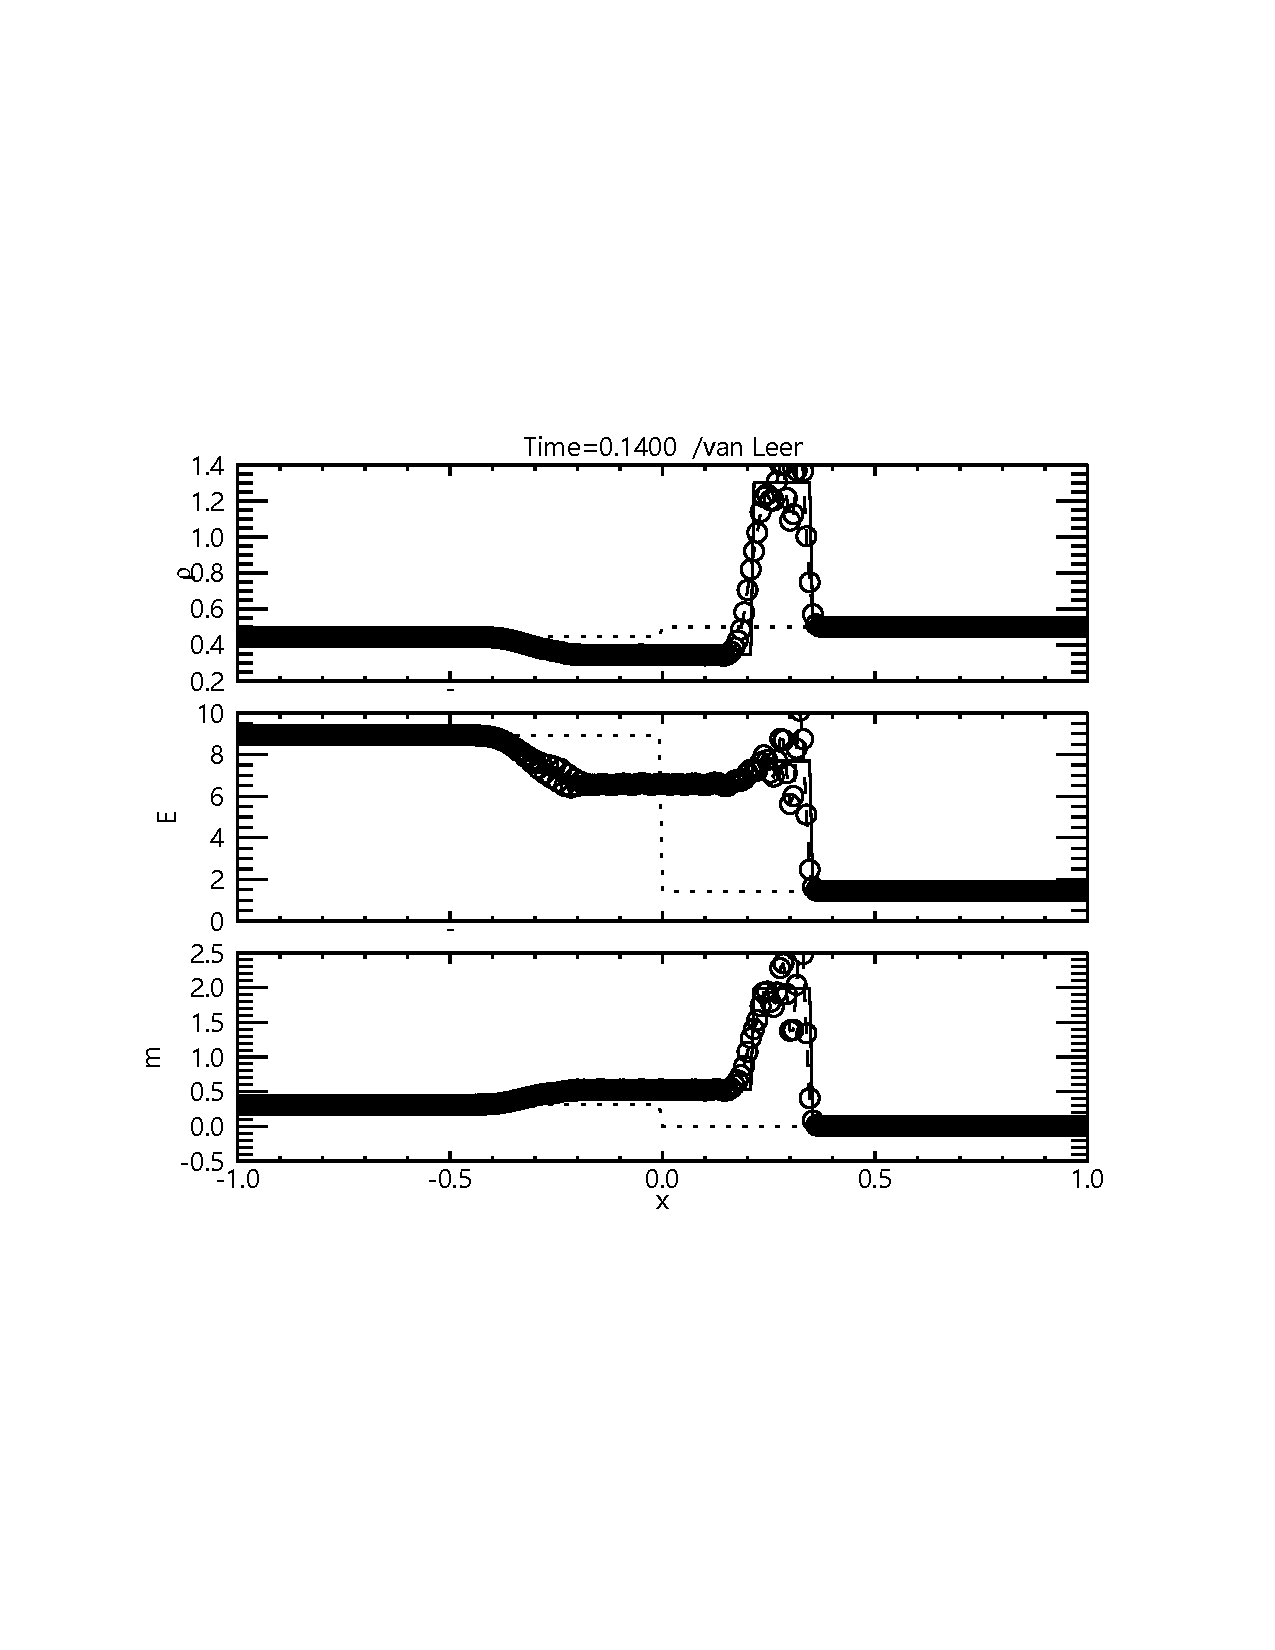
\includegraphics[width=.85\textwidth]{fig_tvd.pdf}
\caption{Lax-Wendroff格式计算结果, 网格点数为 133. \textbf{从上到下分别是密度 $\rho$, 能量 $E$ 和质量流 $m = \rho u$.}
其中点线是初值, 虚线 (上面的数据点用符号 $\circ$ 标注) 是 $t=0.14$ 时的数值结果, 实线是对应的真实解.}\label{Fig:LaxA}
\end{center}
\end{figure}

\begin{figure}
\begin{center}
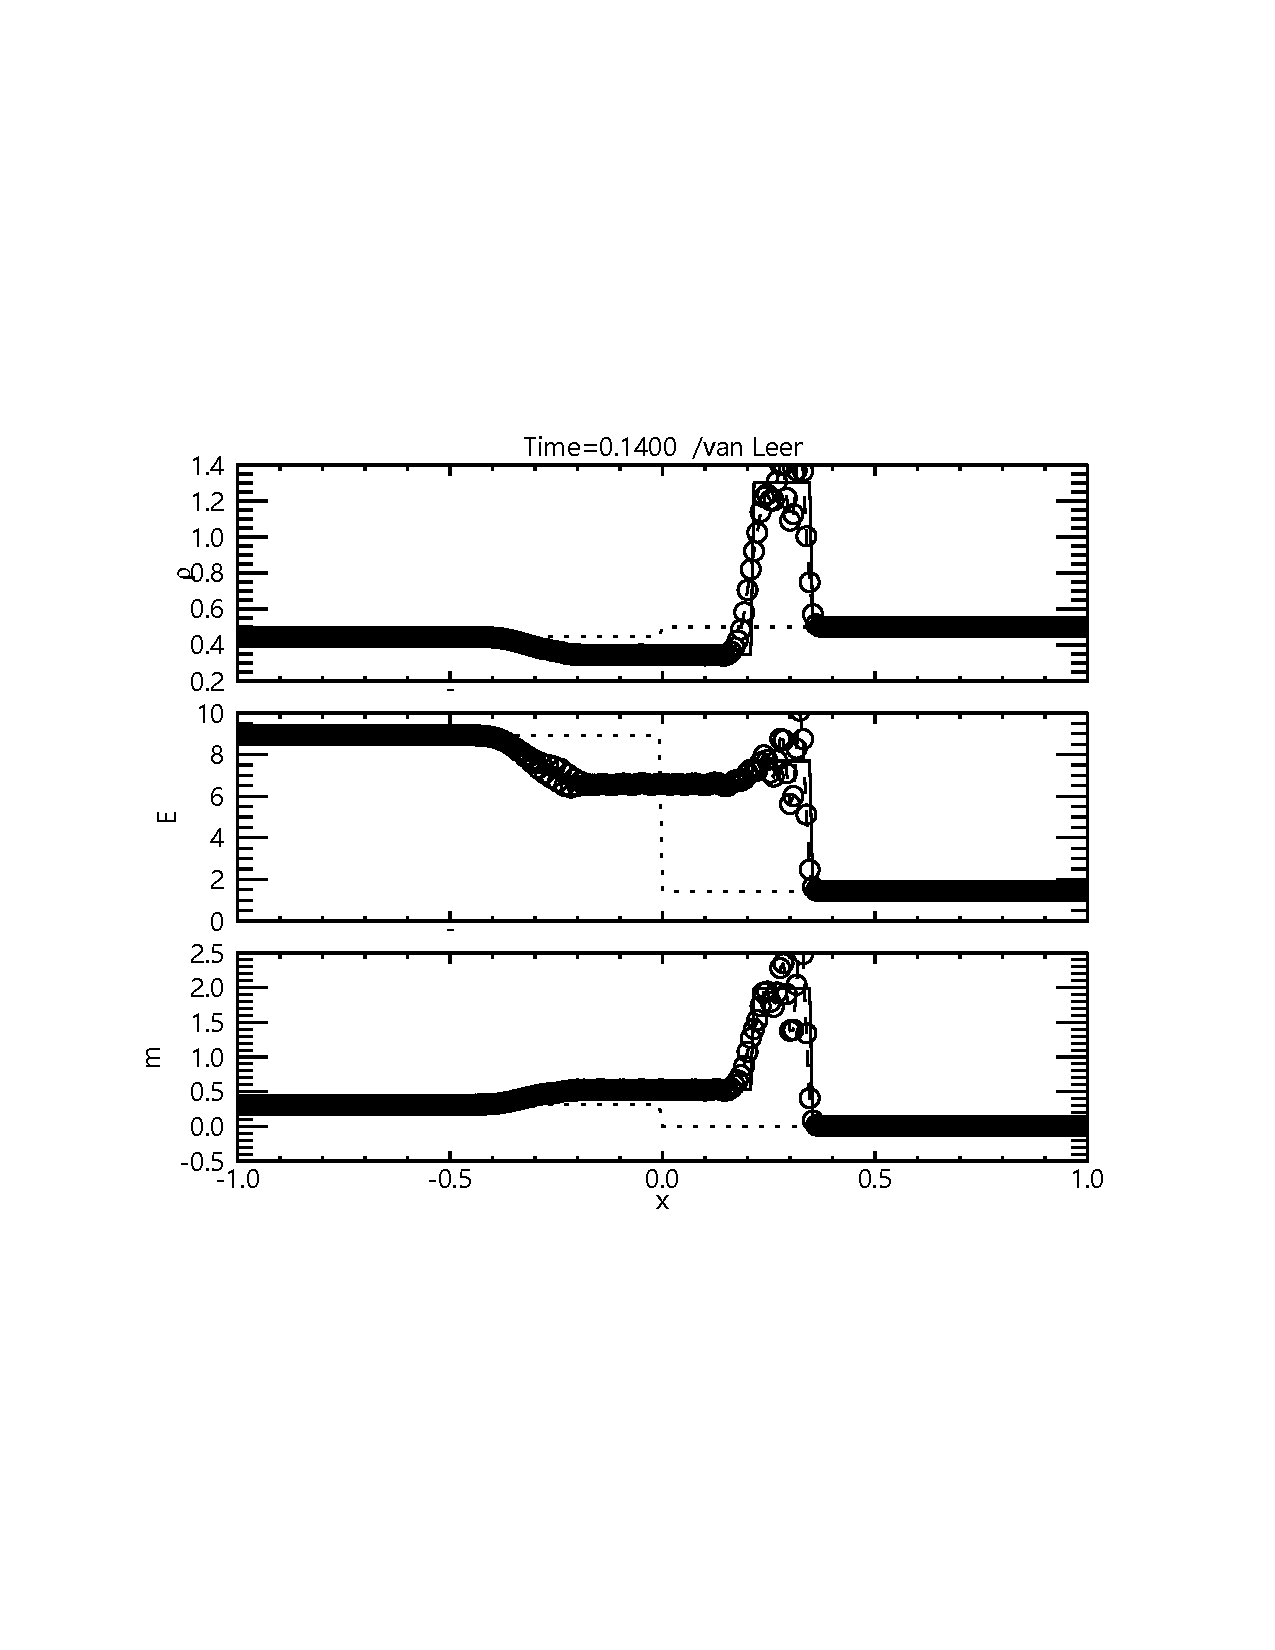
\includegraphics[width=.85\textwidth]{fig_tvd.pdf}
\caption{Lax-Wendrof格式计算结果, 网格点数为 261. 
其他标注同图\ref{Fig:LaxA}.}\label{Fig:LaxB}
\end{center}
\end{figure}

\begin{figure}
\begin{center}
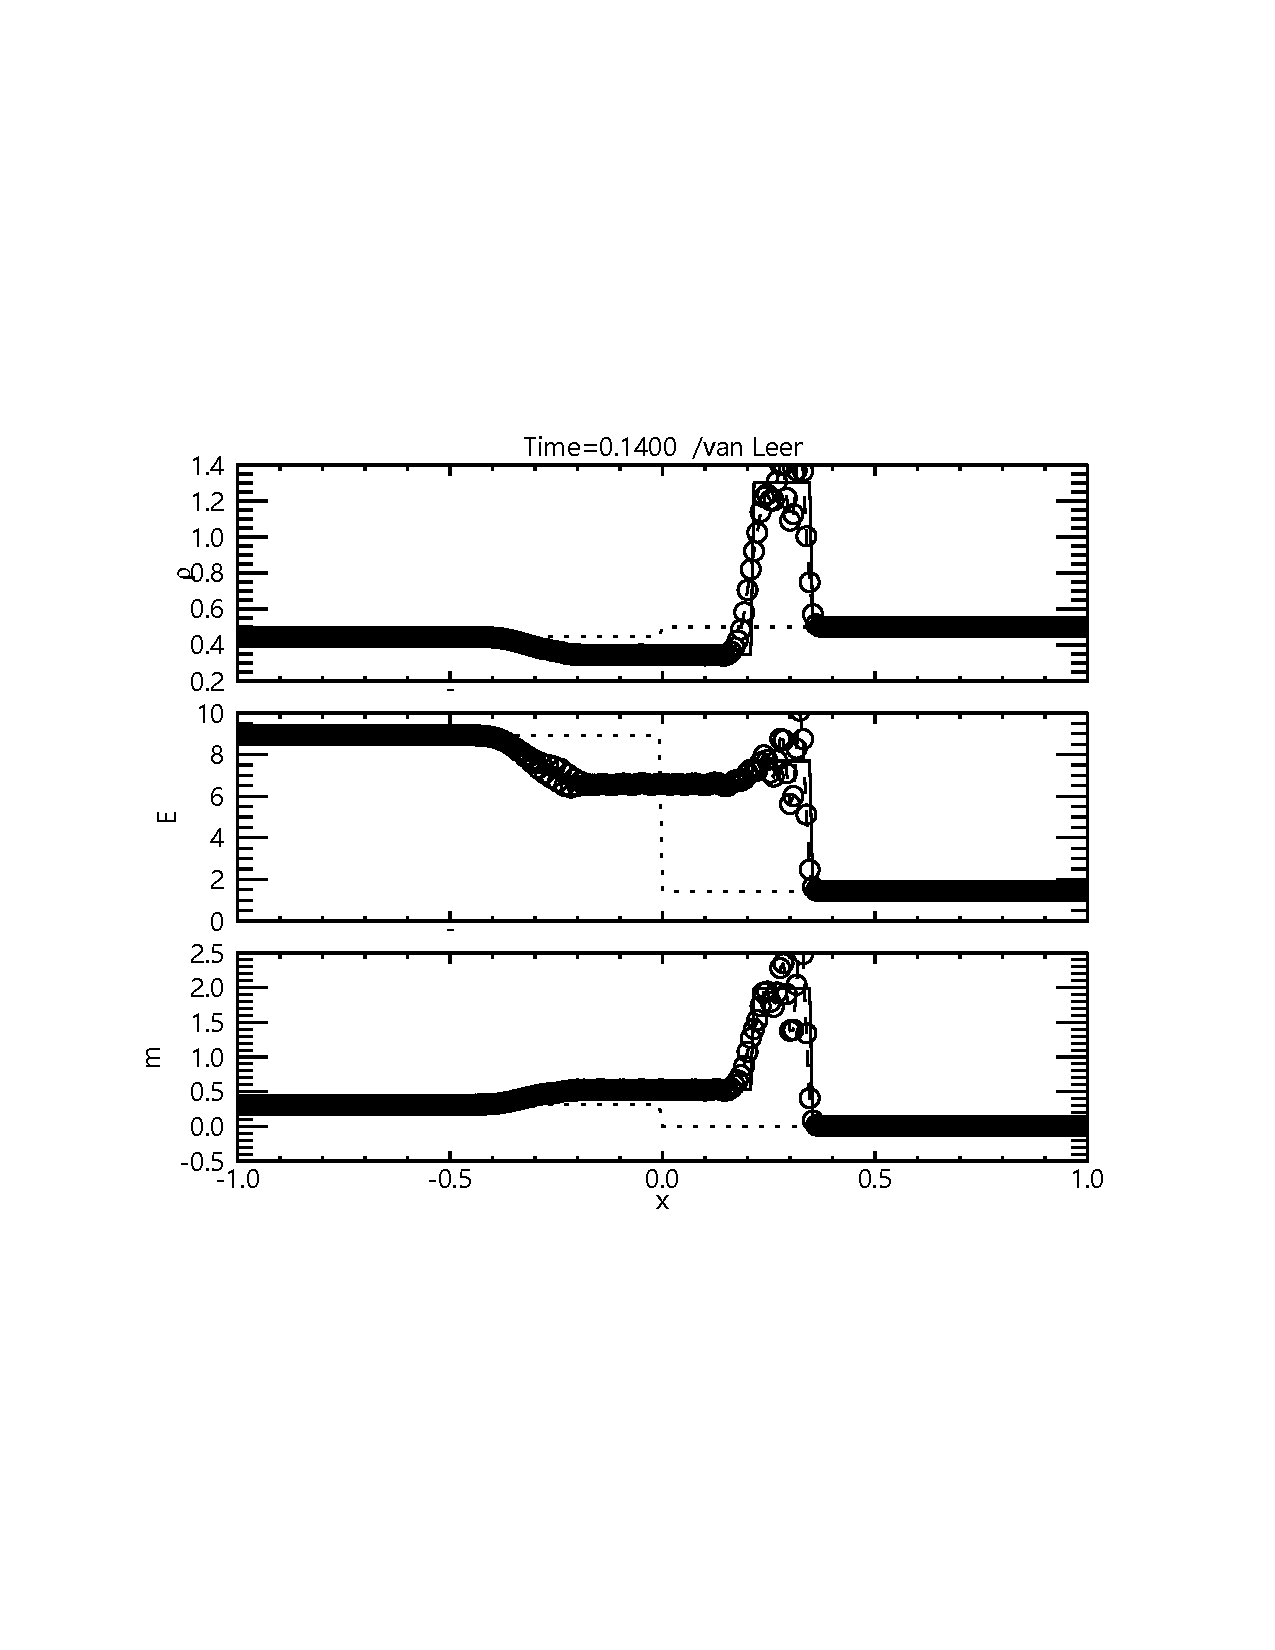
\includegraphics[width=.85\textwidth]{fig_tvd.pdf}
\caption{(van Leer) TVD 格式计算结果, 网格点数为 133. 其他标注同图\ref{Fig:LaxA}.}\label{Fig:vanLeerA}
\end{center}
\end{figure}

\begin{figure}
\begin{center}
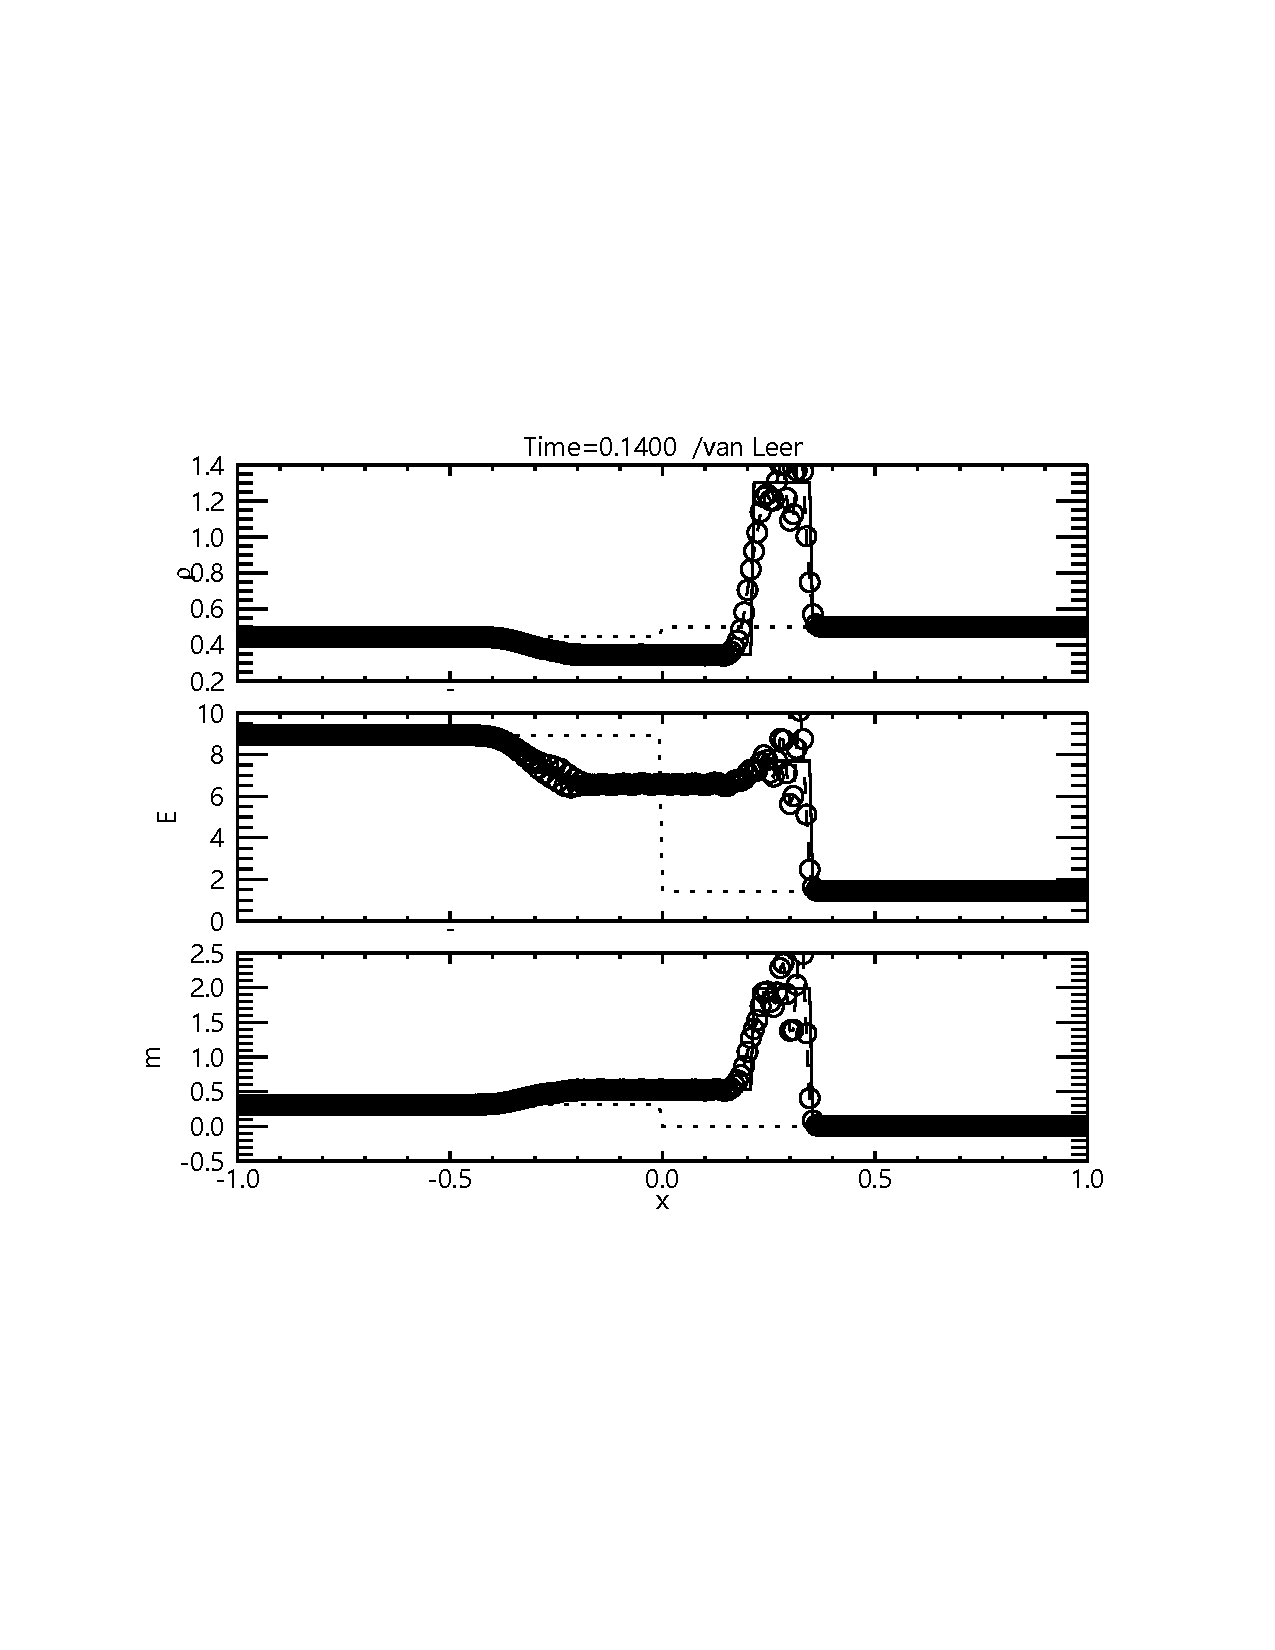
\includegraphics[width=.85\textwidth]{fig_tvd.pdf}
\caption{(van Leer) TVD 格式计算结果, 网格点数为 261. 其他标注同图\ref{Fig:LaxA}.}\label{Fig:vanLeerB}
\end{center}
\end{figure}

\section{格式参考}
\subsection{Lax-Wendroff格式}
对于守恒型方程,
\begin{align}
\frac{\partial u}{\partial t} + \frac{\partial F}{\partial x} = 0,
\end{align}
其Lax-Wendroff格式为
\begin{align}
u_j^{n+1} =& u_j^n - \frac{\Delta t}{2\Delta x} (F_{j+1}^n - F_{j-1}^n) \nonumber\\
& + \frac{\Delta t^2}{2\Delta x^2} \left[A_{j+1/2}^n (F_{j+1}^n-F_j^n) - A_{j-1/2}^n (F_j^n -
F_{j-1}^n)\right]
\end{align}
其中$A = \frac{\partial F}{\partial u}$, $A$的表达式见第\ref{Appendix}节.
\begin{align}
A_{j \pm 1/2}^n = A(u_{j \pm 1/2}^n), \qquad u_{j \pm 1/2}^n = \frac{1}{2} (u_j^n + u_{j \pm 1}^n)
\end{align}

\subsection{TVD格式}
方程
\begin{align}
\frac{\partial u}{\partial t}+\frac{\partial f}{\partial x}+h=0,
\end{align}
令$v_{j+1/2} = V(v_j, v_{j+1})$为$v_j$和$v_{j+1}$的平均值, 
且$\Delta_{j+1/2}v = v_{j+1} - v_j$在坐标空间$\left\{R^k \left(v_{j+1/2}\right)\right\}$的各个分量为$\alpha^{k} _{j+1/2}$
\begin{align}
\Delta_{j+1/2}v =& \sum_k \alpha^{k}_{j+1/2} R^{k}_{j+1/2},\\
\alpha^{k}_{j+1/2} =& L^{k}_{j+1/2} \Delta_{j+1/2}v.
\end{align}
矩阵$A$的特征值为 $u-a$, $u$, $u+a$ ($a^2 = \gamma p/\rho$) 和相应的左右特征向量矩阵为 $L$ 和 $R$, 这里$R$和$L$的表达式见第\ref{Appendix}节.
方程的TVD格式为\citep{Harten1983}
\begin{align}
v_{j}^{n+1}=&v_{j}^{n}-\lambda\left(\bar{f}_{j+1 / 2}^{n}-\bar{f}_{j-1 / 2}^{n}\right)-\Delta t h_{j}^{n}
\\
\bar{f}_{1+1 / 2}=&
\frac{1}{2}\left[f\left(v_{j}\right)+f\left(v_{j+1}\right)\right] \nonumber
\\ &+\frac{1}{2 \lambda} \sum_{k=1}^{5} R_{j+1 / 2}^{k}\left[g_{j}^{k}+g_{j+1}^{k}-Q^{k}\left(\nu_{j+1 / 2}^{k}+\gamma_{j+1 / 2}^{k}\right) \alpha_{j+1 / 2}^{k}\right],
\end{align}
其中$\lambda=\delta t/\delta r$, $\nu_{j+1 / 2}^{k}=\lambda a^k(v_{j+1/2})$ 且
\begin{align}
g_{i}^{k}=& s_{i+1 / 2}^{k} \max \left[0, \min \left(\left|\tilde{g}_{i+1 / 2}^{k}\right|, \tilde{g}_{i-1 / 2}^{k} s_{i+1 / 2}^{k}\right)\right] \\
s_{i+1 / 2}^{k}=&\operatorname{sgn}\left(\tilde{g}_{i+1 / 2}^{k}\right) \\ 
\tilde{g}_{i+1 / 2}^{k}=&\frac{1}{2}\left[Q^{k}\left(\nu_{i+1 / 2}^{k}\right)-\left(\nu_{i+1 / 2}^{k}\right)^{2}\right] \alpha_{i+1 / 2}^{k} \\ 
\gamma_{i+1 / 2}^{k}=&\left\{\begin{array}{ll}{\left(g_{i+1}^{k}-g_{i}^{k}\right) / \alpha_{i+1 / 2}^{k},} & {\text { when } \alpha_{i+1 / 2}^{k} \neq 0} \\ {0,} & {\text { when } \alpha_{i+1 / 2}^{k}=0}\end{array}\right.
\end{align}
其中$Q$的值可以取为
\begin{align}
Q(x)=\left\{\begin{array}{ll}{\frac{x^{2}}{4 \epsilon}+\epsilon,} & {|x|<2 \epsilon} \\ {|x|,} & {|x| \geq 2 \epsilon}\end{array}\right.
\end{align}
其中$0< \epsilon \leq 1/2$, 取$\epsilon=0.1$.


\section{守恒形式方程的特征向量计算}\label{Appendix}
守恒形式下 $A$ 的表达式
\begin{align*}
A =& \frac{\partial f}{\partial w} = \left[\begin{array}{ccc} 0 & 1 & 0
\\
\frac{1}{2} (\gamma  - 3) u^2 & -(\gamma - 3) u & \gamma - 1
\\
(\gamma - 1) u^3 - \gamma \frac{u}{\rho} E & \gamma \frac{1}{\rho} E-\frac{3}{2} (\gamma
- 1) u^2 & \gamma u
\end{array}
\right]
\end{align*}
左右特征向量
\begin{align*}
R =& \left[\begin{array}{ccc} 1 & 1 & 1
\\
u - c & u & u + c
\\
H - u c & \frac{1}{2} u^2 & H + u c
\end{array}
\right]
\\
L =& \frac{\gamma - 1}{2 c^2} \left[\begin{array}{ccc} \frac{1}{2} u \left(u + \frac{2
c}{\gamma - 1}\right) & -\left(u + \frac{c}{\gamma - 1}\right) & 1
\\
2(H - u^2) & 2 u & - 2
\\
\frac{1}{2} u \left(u - \frac{2 c}{\gamma - 1}\right) & -\left(u - \frac{c}{\gamma -
1}\right) & 1
\end{array}
\right]
\end{align*}
其中
\begin{align*}
H =& \frac{E + p}{\rho} = \frac{c^2}{\gamma - 1} + \frac{1}{2} u^2,
\\
c^2 =& \gamma \frac{p}{\rho}.
\end{align*}

\section*{文件清单}
\begin{enumerate}
\item
hw3.tex -- 本报告\LaTeX 文件.
\item
hw3.pdf -- 本报告PDF输出文件.
\item
References.bib -- 文献文件.
\item
fig\_tvd.pdf -- Lax-Wendroff格式计算结果, 133网格.
\item
fig\_tvd.pdf -- Lax-Wendroff格式计算结果, 261网格.
\item
fig\_tvd.pdf -- van Leer TVD格式计算结果, 133网格.
\item
fig\_tvd.pdf -- van Leer TVD格式计算结果, 261网格.
\item 
tvd.pro, hw3\_tvd.pro -- TVD格式计算的IDL程序.
\item 
lax.pro -- Lax-Wendroff格式计算的IDL程序.
\item
Hydrodynamics.xlsx -- 相关问题Excel计算表格, 深绿色单元为输入, 可以变更, 供大家参考. 其中
\begin{enumerate}
\item
Riemann 表格中, B2为$\gamma$值, B4--B6和E4-E6分别是左侧和右侧的密度, 质量流及能量的初值. A25--A26迭代用值, A24为A25和A26的平均值. 22行复制24行的值. 当G24, 即G22值为零时, 得到此 Riemann 问题的解. N3为时间值, 密度, 质量流及能量图形的坐标初值和对应比例分别由N4--N6和O4--O6调节.
\item
Hydrodynamics 表格为对应守恒型方程的矩阵特征值, 左右特征向量, 变量在各个波模的分解, 等等. 这些是后续高精度格式所需要的一些中间结果.
\end{enumerate}
\end{enumerate}

\bibliographystyle{apalike}
\bibliography{References}

\end{document}
